\section{Technology}
A wide range of technologies and methods were used to collect data for this assignment. All of the tracking technologies can be grouped into three categories: devices, mobile apps, and desktop software. Fig.\ref{fig:technology} shows the number of students who used technologies in the given categories. 

\begin{figure}[!t]\centering
	%\begin{wrapfigure}{o}{\textwidth}\centering
	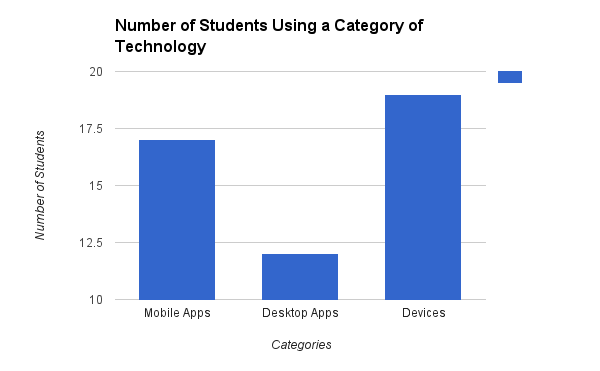
\includegraphics[width=1.0\columnwidth]{images/technology_chart.png}
	\caption{\footnotesize Distribution of technologies used by students\label{fig:technology} 
	}%\end{wrapfigure}
\end{figure}
%

\subsection{Devices}
    The class used numerous devices to keep track of their data for the assignment. Many students used standard devices and manually logged their data into a spreadsheet of some sort. To measure weight, students used a regular scale and logged the data in a spreadsheet. One student used a timer to count their pulse to get their heart rate. Other students used the reportings found on treadmills. 
    Other students used devices that kept track of the data for them. Several students monitored their sleeping patterns using devices like the Garmin Vivofit and the FitBit. These devices track the time it takes to fall asleep, how long the user is sleeping, how many times the user wakes up during the night, and in some cases how long the user is in deep sleep, REM sleep, or light sleep. The data is then uploaded and displayed in some sort of dashboard, usually accessible online. These devices are typically worn on the user as they sleep. The FitBit, for example, is worn on the wrist during sleep. One user used the Garmin  nüvi to keep track of their location with the GPS feature. 

\subsection{Mobile apps} 
    Many users opted to use mobile apps to keep track of their data. Out of the 17 mobile apps used, 13 were iPhone apps and 4 were Android apps. Self reporting apps like Reporter and Lume were used to collect data about the user throughout the day. These apps logged qualitative data about daily aspects of life such as mood, energy, and thoughts. 
    Some of the apps tracked user data automatically. Moment tracked mobile activity on iDevices logging how long a user spent on their phone or iPad throughout the day. Several users used sleep apps similar to the sleep devices mentioned above that tracked various quantitative aspects of sleep. These apps were the Sleep As Android app and the iPhone Sleep Cycle app. Users put their phones on their beds as they slept and the apps tracked things like movement and such. The Galaxy S-Health app was also used to track number of steps and log various health-related aspects of the user’s day to day activities like food intake and stress level.
    
\subsection{Desktop software} 
    Many participants also used desktop software to track their variables. Many users would take a measurement with a device or apparatus that did not automatically record the data and manually log or correct the data themselves, as mentioned above in the devices section. In relation to the FitBit device mentioned above, the FitBit dashboard was used to view data and in some cases manually log data when necessary. Spreadsheets, both Microsoft\textquotesingle s Excel and Google Spreadsheets, were also used to manually log data that was either collected using the devices mentioned above or other data that was not captured using a device. One example of this would be the user that logged the ph of their saliva by using ph test strips and writing their ph level into a spreadsheet. 
    Other students used apps that automatically tracked certain data. Several used apps that monitored their computer usage like TimeStats and Rescue time. These apps kept track of the amount of time spent on certain apps or websites during computer or browser usage. Weather.com was also used to retroactively look up data about the weather and temperatures for the day. Online banking apps were also used to keep track of spending.